\section{Resultados}
A mensagem original foi modulada em frequência, conforme parâmetros na Figura \ref{fig:modulacao}. Os sinais original e modulado podem ser visualizados na Figura \ref{fig:resul_01}. Observa-se que, na modulação em frequência, o sinal original é transformado em uma mensagem que é modulada através da variação da frequência.


\begin{figure}[!htb]
    \centering
    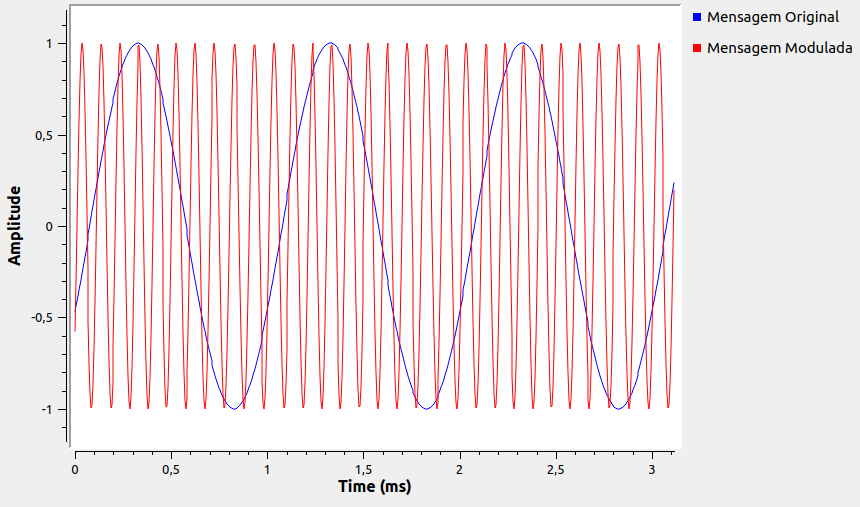
\includegraphics[width=1\linewidth]{Imagens/fig:resul_01.png}
    \caption{sinal original x modulado no tempo}
    \label{fig:resul_01}
\end{figure}

A banda do sinal modulado, Figura \ref{fig:resul_02}, encontra-se utilizando uma largura pequena. Devido a isso, pouco se percebe a alteração da frequência no sinal modulado no domínio do tempo. Porém, conforme se altera o parâmetro $k_f$, é possível verificar a alteração da frequência com mais nitidez. 

\begin{figure}[!htb]
    \centering
    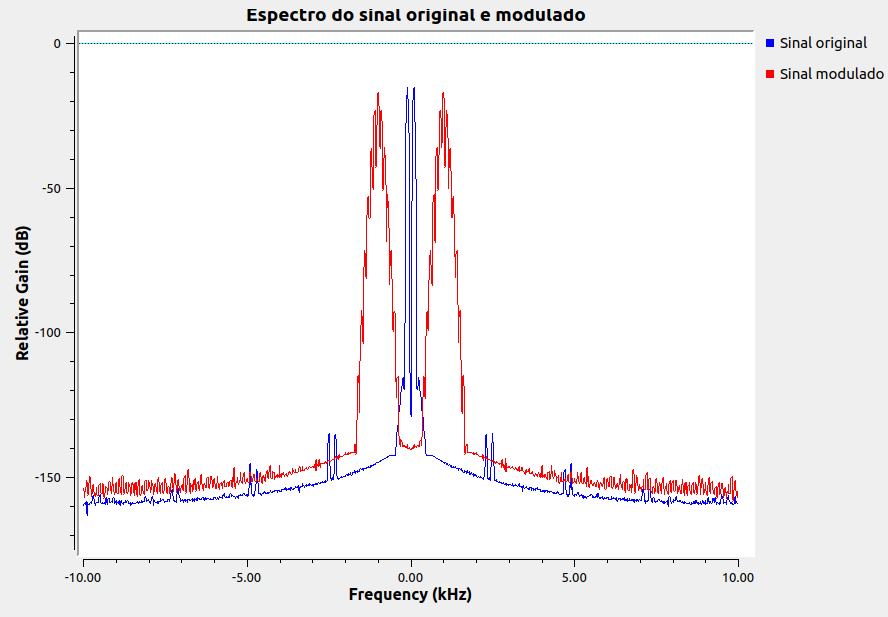
\includegraphics[width=1\linewidth]{Imagens/fig:resul_02.png}
    \caption{espectro do sinal original x modulado}
    \label{fig:resul_02}
\end{figure}

Ao se realizar a conversão FM-AM, o sinal modulado passa a variar em sua amplitude devido à derivada aplicada. Além disso, o sinal modulado é multiplicado por ele mesmo, realizando um deslocamento da banda do sinal para a base. Da mesma forma como em uma modulação AM, há a presença da componente da portadora, o sinal na banda base também se encontra com potência relacionada a portadora.

Na Figura \ref{fig:resul_03}, é possível ver no sinal derivado a alteração da amplitude do sinal e no sinal em banda base, a presença de um \textit{offset} devido à portadora e um sinal mais próximo à mensagem original, também funcionando como um envelope da mensagem. 

\begin{figure}[!htb]
    \centering
    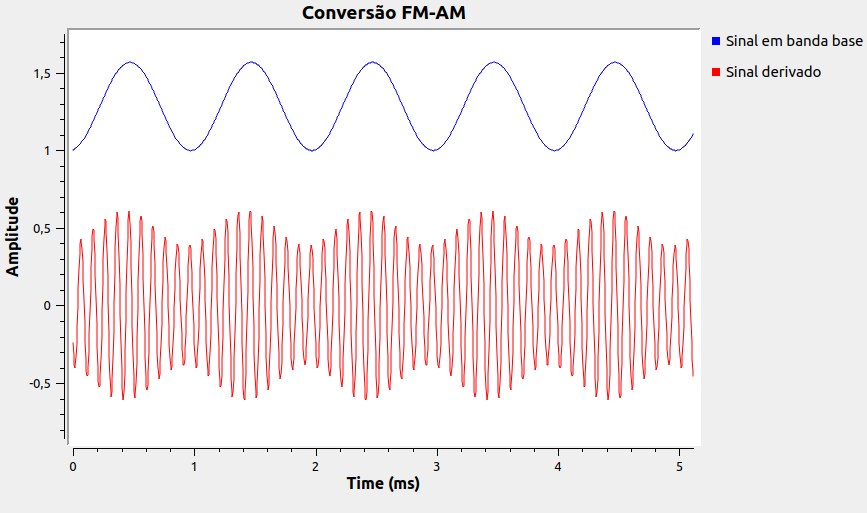
\includegraphics[width=1\linewidth]{Imagens/fig:resul_03.png}
    \caption{conversão FM-AM}
    \label{fig:resul_03}
\end{figure}

O produto do sinal derivado por ele mesmo desloca a banda para a banda base. Na Figura \ref{fig:resul_04}, fica evidente esse deslocamento. 

\begin{figure}[!htb]
    \centering
    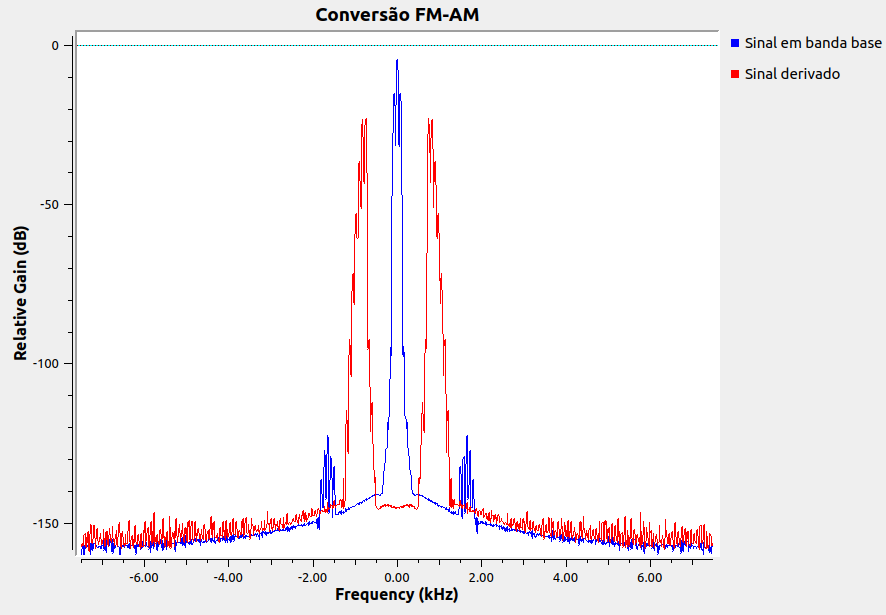
\includegraphics[width=1\linewidth]{Imagens/fig:resul_04.png}
    \caption{espectro do sinal derivado e da banda base}
    \label{fig:resul_04}
\end{figure}

Após a conversão do sinal FM em AM, realiza-se uma demodulação AM no sinal. Ou seja, aplica-se um filtro passa-baixas para isolar a banda base. Dessa forma, obteve-se uma mensagem estimada que se assemelha à mensagem original, Figura \ref{fig:resul_05}.

\begin{figure}[!htb]
    \centering
    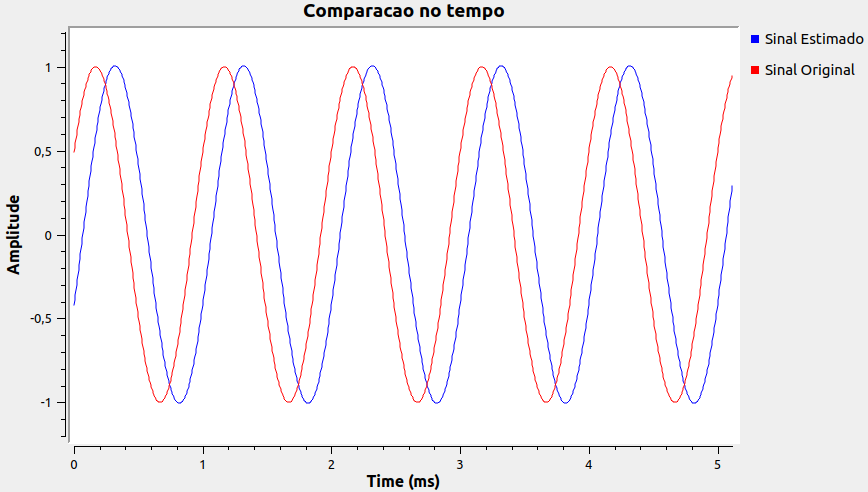
\includegraphics[width=1\linewidth]{Imagens/fig:resul_05.png}
    \caption{sinal original e estimado no tempo}
    \label{fig:resul_05}
\end{figure}

O espectro do sinal original e do demodulado se encontram bastante semelhantes após a demodulação. Atenuação das componentes adjacentes podem ser otimizadas com a otimização dos parâmetros de filtragem escolhidos para o procedimento. 

\begin{figure}[!htb]
    \centering
    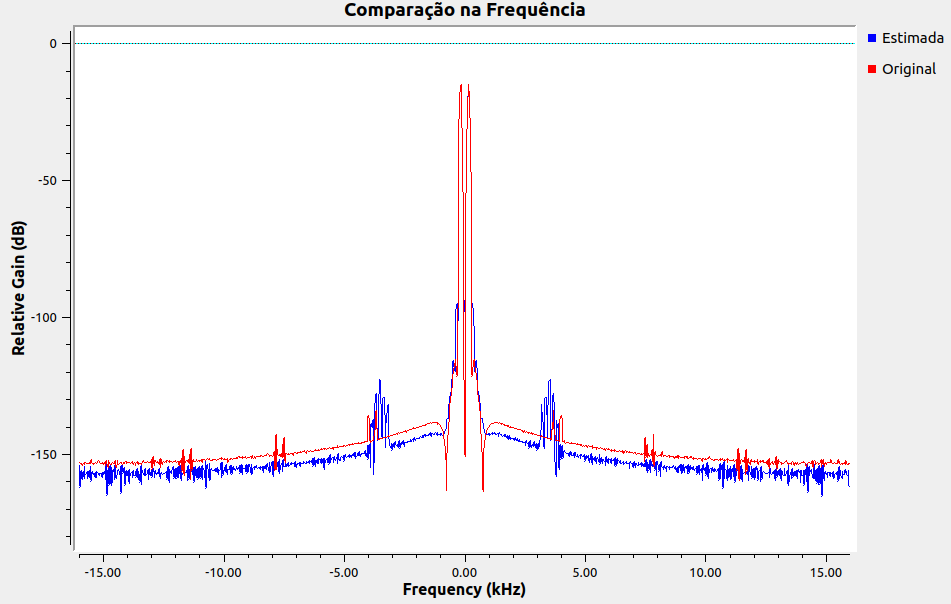
\includegraphics[width=1\linewidth]{Imagens/fig:resul_06.png}
    \caption{espectros do sinal original e demodulado}
    \label{fig:resul_06}
\end{figure}
